\documentclass{beamer}
\usepackage{pgfpages}
\usepackage{amsmath}
\usepackage{amsfonts}
\usepackage{fontspec}
\usepackage{xunicode}
\usepackage{xltxtra}
\usepackage{color}

\usepackage{beamertheme_atilla/beamerthemeAtilla}

\defaultfontfeatures{Mapping=tex-text}
%\setromanfont{Linux Libertine O}
\setsansfont{FreeSans}

\setbeameroption{show notes}
\setbeameroption{show notes on second screen=left}

% Hack to allow XeTeX to produce wide pdf
\renewcommand\pgfsetupphysicalpagesizes{%
	\pdfpagewidth\pgfphysicalwidth\pdfpageheight\pgfphysicalheight%
}

% CUSTOM COLORS ===============================================================

\definecolor{gray}{rgb}{0.5,0.5,0.5}
\definecolor{darkgreen}{rgb}{0.0,0.5,0.0}
\definecolor{mygreen}{rgb}{0,0.6,0}
\definecolor{mygray}{rgb}{0.5,0.5,0.5}
\definecolor{mymauve}{rgb}{0.58,0,0.82}
\definecolor{myorange}{RGB}{246,177,50}

% CUSTOM COMMANDS =============================================================

\newcommand\fixme{\textrm{\textbf{\textcolor{red}{FIXME: }}}}
\newcommand\todo{\textrm{\textbf{\textcolor{myorange}{TODO: }}}}
\newcommand\okeanos{\raise.17ex\hbox{$\scriptstyle\sim$}okeanos }
\newcommand\spc{\hfill \\}
\newcommand\dspc{\spc\spc}

\AtBeginSection[]
{
	\begin{frame}
		\frametitle{Table of Contents}
		\tableofcontents[currentsection]
	\end{frame}
}

% PRESENTATION SETTING ========================================================

\author{Αλέξιος Πυργιώτης}
\title{Σχεδίαση και Υλοποίηση Μηχανισμού Κρυφής Μνήμης για
	Κατανεμημένο Σύστημα Αποθήκευσης σε Περιβάλλον
	Υπολογιστικού Νέφους}
\institute{Εθνικό Μετσόβιο Πολυτεχνείο}
\date{\today}


\begin{document}
\begin{frame}[t,plain]
\titlepage
	\note[item]{Καλημέρα σας, ονομάζομαι Αλέξιος Πυργιώτης\\
		Θα σας παρουσιάσω τη διπλωματική μου με τίτλο:..}
	\note[item]{Ακούγεται κάπως περίεργο στα ελληνικά...\\
	αυτό που πραγματεύται είναι την δημιουργία ενός caching μηχανισμού για 
	το Archipelago, ένα distibuted, storage layer}
	\note[item]{Συγκεκριμένα, στην παρουσίαση αυτή θα μιλήσουμε για τον 
		cached, δηλαδή τον caching μηχανισμό μας και αντικείμενο της 
		διπλωματικης, αλλά και για το synapsed, ένα συμπληρωματικό 
		εργαλείο που στόχος του είναι να δώσει στον cached δικτυακές 
		δυνατότητες}
	\note[item]{Σημείωση: Για οικονομία του λόγου, δε θα προβώ σε εξήγηση 
		βασικών όρων όπως VMs, storage. Παρ'όλα αυτά όμως, αν κάποια 
		από αυτές τις έννοιες είναι άγνωστες ή για όποια απορία κατά τη 
		διάρκεια της παρουσίασης, μπορείτε να με διακόψετε και να 
		ρωτήσετε.}
	
\end{frame}

\begin{frame}[t]{Contents}

	\tableofcontents

	\note[item]{O κορμός της παρουσίασης είναι ο εξής:
		\begin{itemize}
			\item Αρχικά, παρουσιάζουμε κάποια εισαγωγικά που 
				αφορούν το background της εργασίας μας.  
				Αναφέρουμε τι είναι το Synnefo και τι είναι η 
				υπηρεσια ~okeanos
			\item Έπειτα, μιλαμε για τον τρόπο που διαχειριζόμαστε 
				το storage και κατ'επέκταση για το archipelago 
				και τον στόχο της διπλωματικής.
			\item Στη συνέχεια μιλάμε για το τι είναι caching και 
				αναφέρουμε κάποιες σύγχρονες λύσεις για 
				caching.
			\item Τα επόμενα δυο κεφάλαια έχουν να κάνουν με τον 
				cached, και συγκεκριμένα με την παρουσίαση της 
				σχεδίασής του και της απόδοσής του
			\item Αντίστοιχα παρουσιάζουμε το synapsed, τη σχεδίαση 
				και υλοποίησή του
			\item Τέλος, συνοψίζουμε όσα ειπώθηκαν παραπάνω και 
				μιλάμε για μελλοντικές εργασίες
		\end{itemize}
	}

\end{frame}

\section{Introduction}

\begin{frame}{Synnefo}
	\note{Ας ξεκινήσουμε με την παρούσα κατάσταση.\\
	Το software που τα ξεκίνησε όλα είναι το Synnefo}

	
\includegraphics{images/synnefo-logo.png}

	Open source, production-ready, cloud software.\\
	Designed since 2010 by GRNET.
	\note{\dspc..by GRNET -> Και φυσικά τα παιδιά που βλεπετε εδώ}
	
	\spc
	Synnefo, as most cloud software, has the following services:
	\begin{itemize}
		\item Compute Service
		\item Network Service
		\item Storage Service
		\item Image Service
		\item Identity Service
	\end{itemize}

	\note{\dspc
		\begin{itemize}
			\item Compute service, είναι η υπηρεσία η οποία 
				προμηθεύει τους χρήστες με VMs και επιτρέπει το 
				χειρισμό τους
			\item Network service, είναι η υπηρεσία η οποία δίνει 
				τη δυνατότητα στους χρήστες να δημιουργήσουν 
				ιδιωτικά δίκτυα και να συνδέσουν τα VMs τους σε 
				αυτά.
			\item Storage service, που παρέχει αποθηκευτικό χώρο 
				στους χρήστες.
			 \item Image Service, υπεύθυνο για το deployment ενός 
				 VM από ένα image.  Επίσης, κάνει και 
				 παραμετροποιήσεις (παράδειγμα ssh κλειδιά)
		\end{itemize}
	}
\end{frame}

\begin{frame}{okeanos}

	
\includegraphics{images/okeanos-logo.png}

	\begin{itemize}
		\item IaaS service
		\item Targeted at the Greek Academic and Research Community
		\item Designed by GRNET
		\item In production since 2011
	\pause
		\item ...and of course powered by Synnefo.
	\end{itemize}

	\note{
		\begin{itemize}
			\item IaaS είναι πρακτικά η παροχή εικονικής υποδομής 
				σε χρήστες (δηλαδή πάρε υπολογιστή (VM), 
				δίκτυα, αρχεία κτλ)
			\item Δωρεάν για τους Ακαδημαϊκους σκοπούς, ήδη 
				γίνονται εργαστήρια στο EMP και απ' αυτό το 
				εξάμηνο σε άλλες σχολές
			\item \click
			\item Και φυσικά παίζει πάνω σε Synnefo...
		\end{itemize}
	}
				
\end{frame}



\section{Request handling}

\begin{frame}[t]{What is request handling?}

	\note{Τι είναι η διαχείριση των αιτημάτων ενός VM?\\
		Είναι η εφαρμογή πολιτικών και επεξεργασία των αιτημάτων σε όλη 
		την πορεία τους μέχρι το να φτάσουν στο storage.\dspc
		Δηλαδή έχουμε ένα εικονικό μηχάνημα <κλικ>\\
		... το storage μας <κλικ>\\
		και πρέπει με κάποιο τρόπο τα δεδομένα του μηχανήματος να 
		φτάσουν σε εμάς <κλικ>\\

		Ένας απλός τρόπος θα ήταν να τα συνδέσουμε. Άλλωστε όταν τρέχει 
		VM, ο hypervisor κοιτάει block device. Θα μπορούσε να ήταν 
		κομμάτι του storage
		Είναι αυτό αρκετό; <κλικ>\\
		Όχι, χρειαζόμαστε επίσης \fixme
	}


	\begin{columns}[t]
		\begin{column}{.5\textwidth}
			\pause
			\makebox[\textwidth]{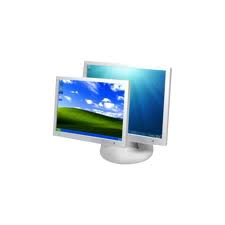
\includegraphics[width=.2\paperwidth]{images/vm.jpg}}
			\pause \centering{ {\Huge +} }
				\makebox[\textwidth]{
\includegraphics[width=.2\paperwidth]{images/cloud-server1.jpg}}
			\pause \centering{ {\Huge = ?}}
		\end{column}
		\begin{column}{.5\textwidth}
			\pause
			\begin{itemize}
				\item Policy enforcement?
				\item Storage agnosticity?
			\end{itemize}
		\end{column}
	\end{columns}

\end{frame}

\begin{frame}{Our solution}

	{\Large Archipelago}

	\makebox[\textwidth]{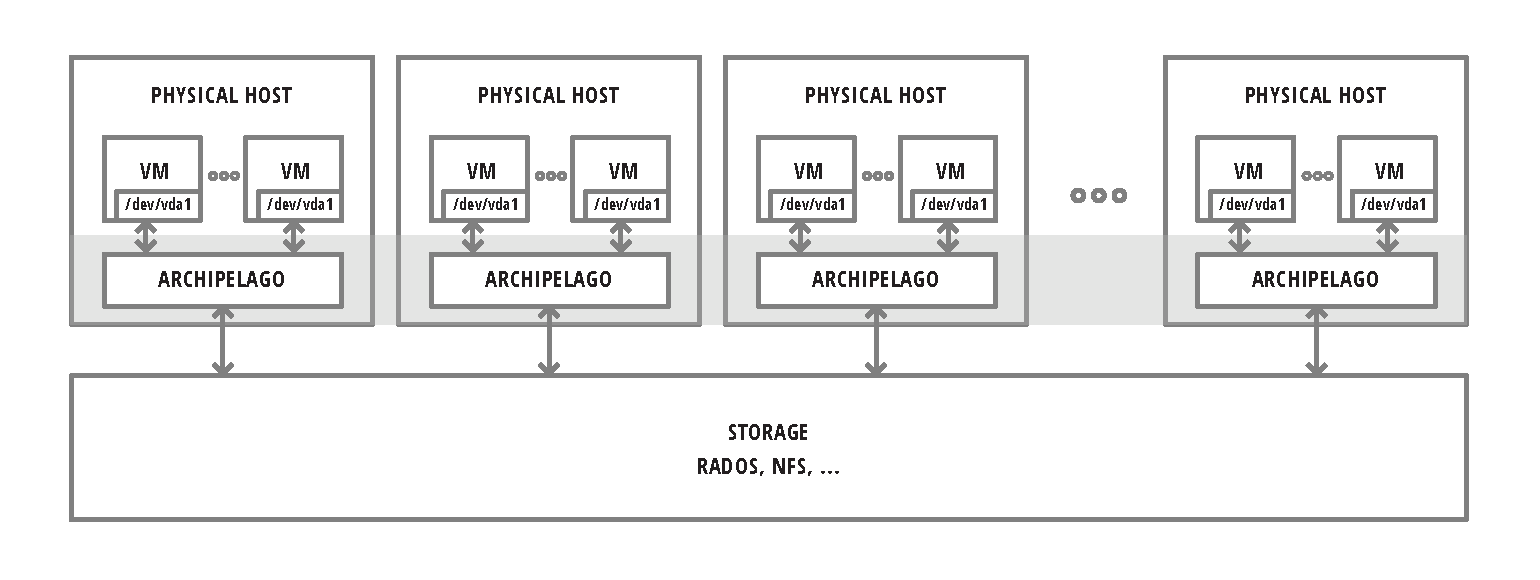
\includegraphics[width=\textwidth]{images/archipelago_overview_a.pdf}}

	\spc

	Key features:
		1) Software-defined
		2) Distributed
		) Modular
		Copy-On-Write
		Storage agnostic

	\note{Η λύση που χρησιμοποιήσαμε είναι το Archipelago}
	\note{
		\begin{itemize}
			\item Software-defined: αν και είναι ένα όρος 
				μαρκετινγκ, εμείς κανονικά. Σημαίνει με το 
				software ΟΡΙΖΕΙΣ το storage (εφαρμογή policy, 
				αλλαγή πορείας του request)
			\item τρέχει σε πολλούς κόμβους
			\item αποτελείται από διακριτά κομμάτια
			\item κάνει CoW (εξήγησε ότι τα images είναι λίγα, τα
				VMs πολλά, όπως όταν ένα process κάνει fork)
			\item μπορούμε χρησιμοποιήσουμε ότι θέλουμε
		\end{itemize}
	}

\end{frame}

\begin{frame}{Archipelago Architecture}
	%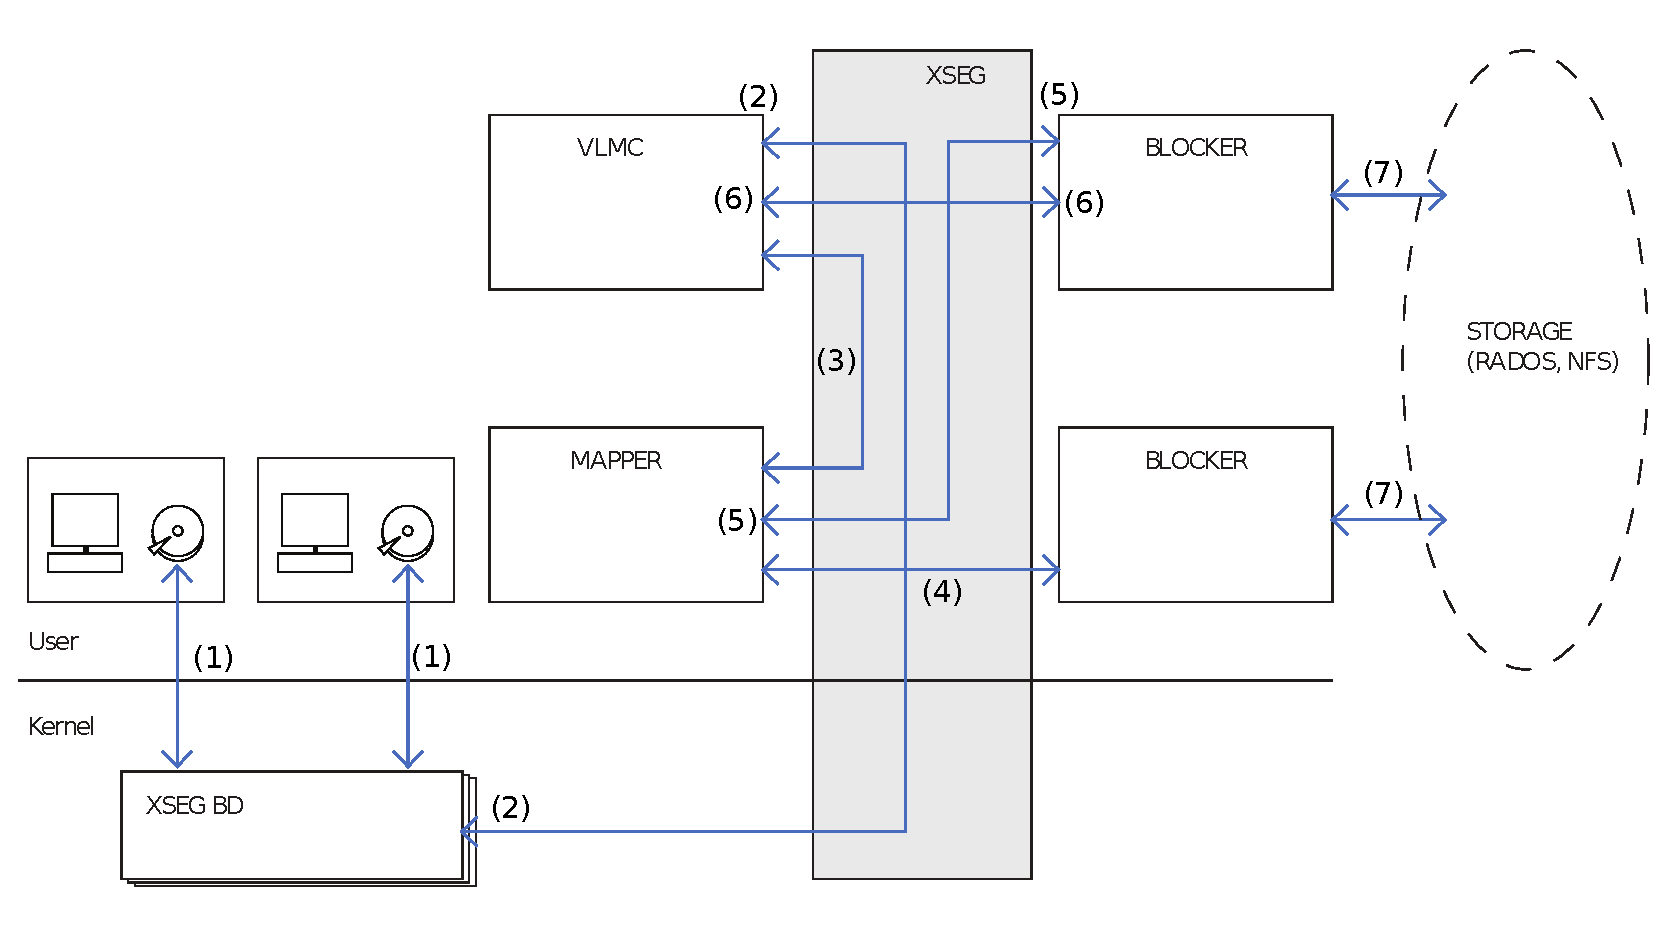
\includegraphics[{images/new_sxima_numbered.pdf}
	\begin{center}
		  \makebox[\textwidth]{\includegraphics[width=0.9\paperwidth]{images/new_sxima_numbered.pdf}}
	\end{center}

	\note[item]{To VM στέλνει αίτημα στο δίσκο του, ο δίσκος είναι εικονικός, 
		θα το δει ο hypervisor (εξήγησε τι είναι ο hypervisor) και θα το 
		στείλει στον δίσκο που το έχουμε πει. (xsegbd)}
	\note[item]{Ο xsegbd στέλνει τo αίτημα στο userspace κομμάτι του 
		Αρχιπελάγους το οποίο αποφαίνεται για τα αντικείμενα τα οποία 
		αντιστοιχούν στο αίτημα}
	\note[item]{μετά τα ζητάει από το storage μέσω των blockers}
\end{frame}

\begin{frame}{RADOS}

	The object store component of Ceph filesystem.\\
	\spc
	Key features:
	\begin{itemize}
		\item Replication
		\item Fault tolerance
		\item Self-management
		\item Scalability
	\end{itemize}


	\pause

	\spc
	Speed issues:\\
	VM with page-cache: > 90MB/s, < 1ms\\
	VM without page-cache: < 7MB/s, ~ 10ms

	\pause

	\spc
	Thesis goal: make this faster.

\end{frame}


\section{Caching}

\begin{frame}{Intro}

	Solution: Caching\\
	\spc
	Caching is:
	\begin{itemize}
		\item We have a slow medium
		\item Add a fast medium in a data path
		\item Transparently store the data that are intended for the 
			slower medium.
		\item Profit: later accesses to the same data are faster
	\end{itemize}
	\dspc
	Sounds familiar?
\end{frame}

\begin{frame}
	\makebox[\textwidth]{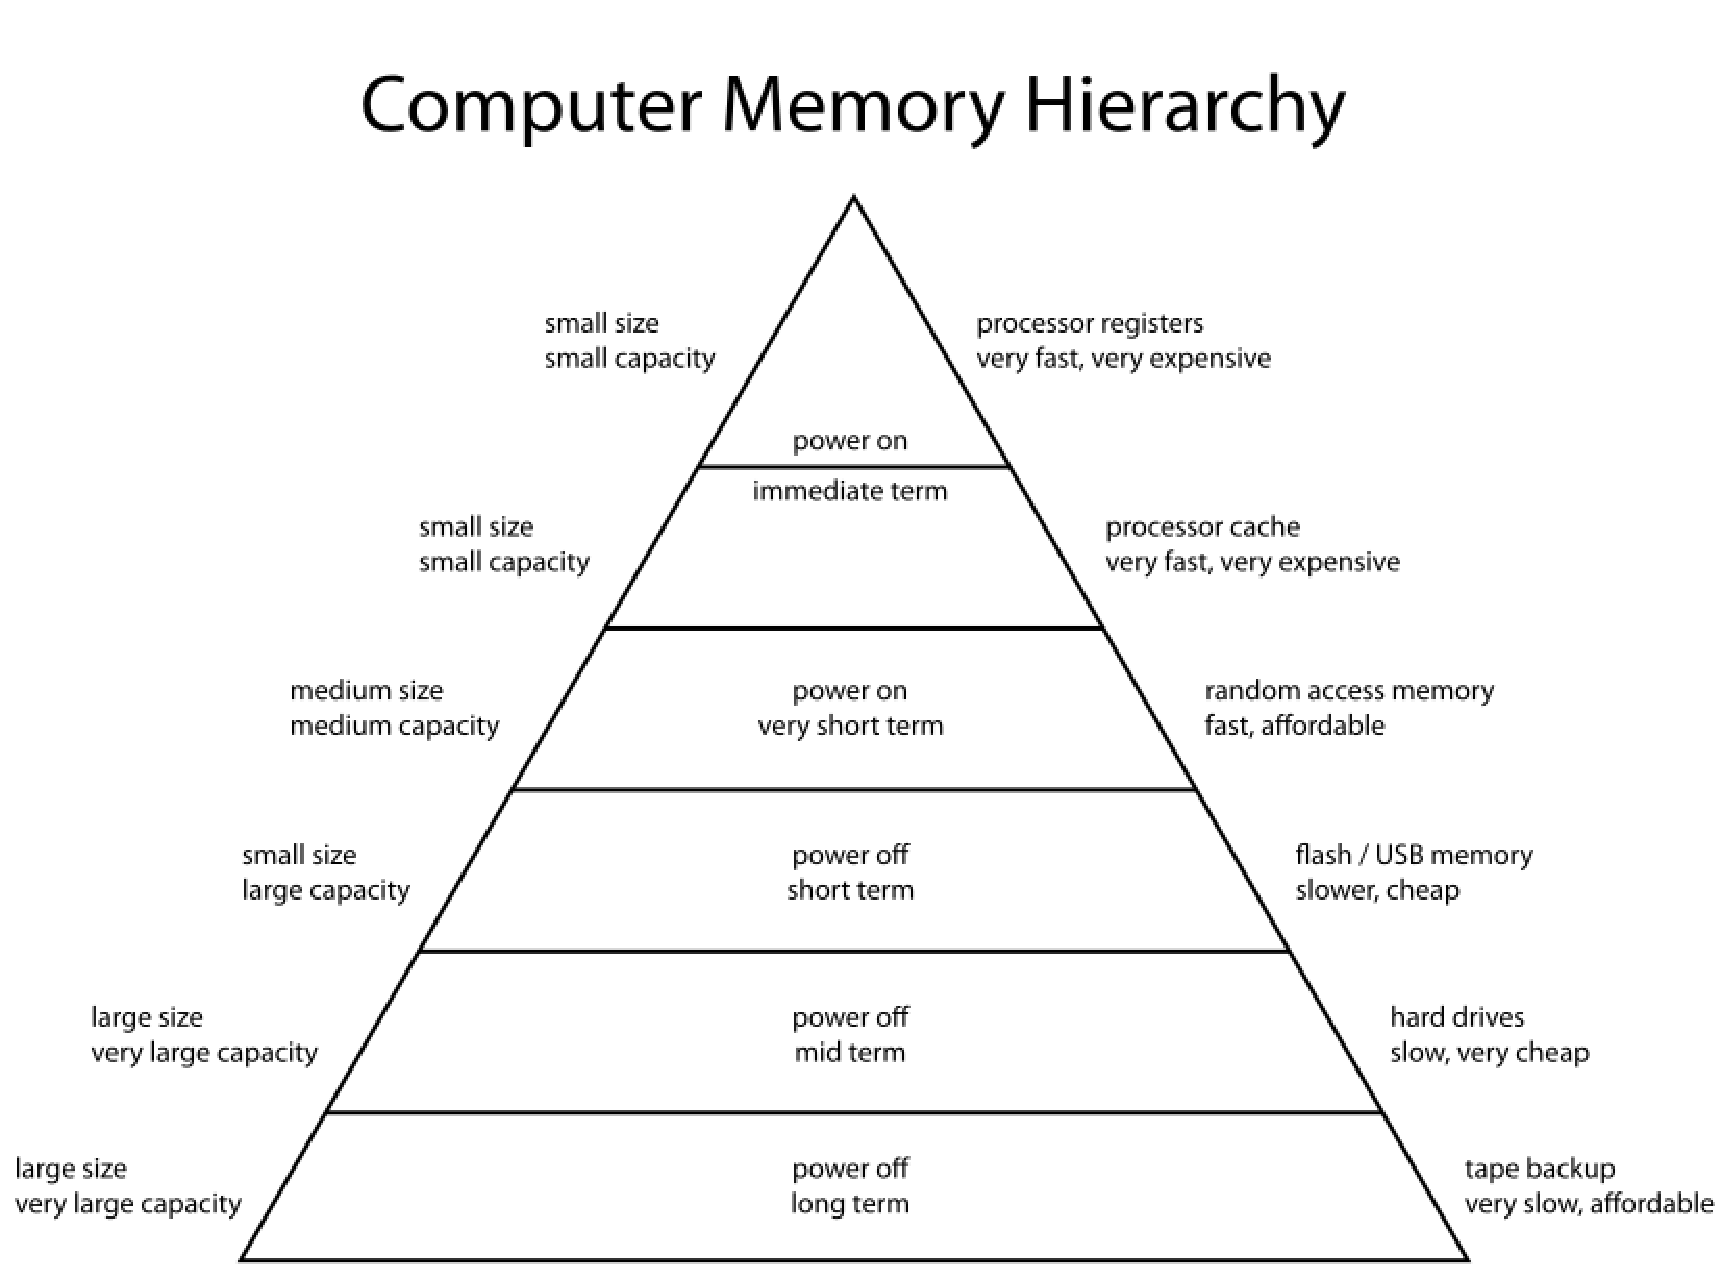
\includegraphics[width=0.8\textwidth]{images/mem-hier.pdf}}
	
	That's because every PC is built that way.
\end{frame}

\begin{frame}
	Is there anything to help us?
	\dspc
	We are not the first to have speed issues
	\dspc
	Facebook, Twitter, Dropbox, every one has hit and surpassed their 
	limits.
	\dspc
	There are solutions separated in two categories:
	\begin{itemize}
		\item Block store
		\item Key-value store
	\end{itemize}
\end{frame}

\begin{frame}{Block-store caching solutions}

	Most notable examples:
	\begin{itemize}
		\item Bcache
		\item Flashcache
		\item EnhanceIO
	\end{itemize}
	\dspc
	Typically scale-up solutions.
	\dspc
	Pros: Simple, scale-up\\
	Cons: Unaware of CoW, kernel solutions
\end{frame}

\begin{frame}{Key-value caching solutions}
	Most notable examples:
	\begin{itemize}
		\item Memcached
		\item Couchbase
	\end{itemize}
	\dspc
	Typically scale-out solutions
	\dspc
	Pros: Distributed with no SPOF, can utilize unneeded RAM\\
	Cons: Memcached has no persistence, Couchbase cannot use RADOS as its 
	backend, more suitable for databases
\end{frame}

\begin{frame}{Page-cache}

	What if we used the page-cache?

	\dspc
	Pros: Easy to activate, tested, very fast\\
	Cons: Unaware of CoW, no control over it, practically kernel solution\\

\end{frame}

\begin{frame}{Conclusions}

	\begin{itemize}
		\item Most solutions far from Archipelago's logic
		\item Block store might be good for the storage backend
		\item Must implement our own solution
	\end{itemize}
\end{frame}
	

\section{Cached design}

\begin{frame}{Requirements}

	Design goals for cached:
	\begin{itemize}
		\item Create something close to the Archipelago logic
		\item Measure the best possible performance we can get
	\end{itemize}
	\dspc
	Stricter requirements for cached:
	\begin{itemize}
		\item Nativity
		\item Pluggability
		\item In-memory
		\item Low indexing overhead
	\end{itemize}
\end{frame}

\begin{frame}{Cached design}
	operations image

	component image
\end{frame}

\begin{frame}{Xcache design}
	show with red the xcache design

	go to xcache picture

	Show what xcache does
\end{frame}

\begin{frame}{Xworkq design}
	show the xworkq design

	what xworkq does
\end{frame}

\begin{frame}{Xwaitq design}
	show xwaitq design

	what xwaitq does
\end{frame}

\begin{frame}{Bucket pool}
	Buckets have been designed to do this	

	list
\end{frame}



\end{document}

